\documentclass[11pt,twoside]{article}

\usepackage{paperlighter}

\usepackage{longtable, setspace, outlines}
 % for OliveGreen
\definecolor{OliveGreen}{rgb}{0,0.6,0}
% Set link colors
%\usepackage[rgb,dvipsnames]{xcolor}
%\hypersetup{colorlinks=true, linkcolor=RoyalBlue, urlcolor=RoyalBlue}

\usepackage{pdfpages} % for includepdf


% Recommended, but optional, packages for figures and better typesetting:
\usepackage{microtype}
\usepackage{graphicx}
\usepackage{subfigure}
\usepackage{booktabs} % for professional tables

% Attempt to make hyperref and algorithmic work together better:
\newcommand{\theHalgorithm}{\arabic{algorithm}}


% For theorems and such
\usepackage{amsmath}
\usepackage{amssymb}
\usepackage{mathtools}
\usepackage{amsthm}

% if you use cleveref..
\usepackage[capitalize,noabbrev]{cleveref}

%%%%%%%%%%%%%%%%%%%%%%%%%%%%%%%%
% THEOREMS
%%%%%%%%%%%%%%%%%%%%%%%%%%%%%%%%
\theoremstyle{plain}
\newtheorem{theorem}{Theorem}[section]
\newtheorem{proposition}[theorem]{Proposition}
\newtheorem{lemma}[theorem]{Lemma}
\newtheorem{corollary}[theorem]{Corollary}
\theoremstyle{definition}
\newtheorem{definition}[theorem]{Definition}
\newtheorem{assumption}[theorem]{Assumption}
\theoremstyle{remark}
\newtheorem{remark}[theorem]{Remark}

% Todonotes is useful during development; simply uncomment the next line
%    and comment out the line below the next line to turn off comments
%\usepackage[disable,textsize=tiny]{todonotes}
\usepackage[textsize=tiny]{todonotes}

% Chinese
\usepackage{xeCJK} % for Chinese, compiling by XeLaTex
\usepackage{indentfirst}
\setlength{\parindent}{2em}  % setting the indentation to be two Chinese characters size.
\usepackage{fontspec} %設定字體
% Fandol font (the default)  not shown "內"
\setCJKmainfont{AR PL UMing TW MBE} % AR PL UMing TW MBE or "UKai" https://www.overleaf.com/learn/latex/Questions/Which_OTF_or_TTF_fonts_are_supported_via_fontspec%3F#Chinese
%BiauKai} %標楷體 from macOS %設定中文為系統上的字型,而英文不去更動,使用原TeX字型
%\setCJKmainfont[Vertical=RotatedGlyphs]{AR PL UMing TW MBE}


\slimtitle{居家牙醫醫療服務} %Paperlighter Example}
\slimauthor{Author 萬芳牙科}


\begin{document}

\lightertitle{居家牙醫醫療服務}

\lighterauthor{祁力行$^{\dagger}$, 李勝揚$^{\ddagger}$}

\lighteraddress{$^\dagger$}{臺北市立萬芳醫院牙科部口腔顎面外科}
\lighteraddress{$^\ddagger$}{臺北市立萬芳醫院牙科部}


\lighteremail{110050@w.tmu.edu.tw}


%\begin{abstract}
摘要:
「身心障礙者口腔照護指導員」訓練課程,多年的臨床工作,許多患者朋友從自行前來就醫,到現在由全家總動員推著輪椅來就醫,生活打理也漸漸需要他人代勞,甚至基本的口腔衛生照護,也面臨須由家人或照護者協助完成;平常在醫學中心,時常會有加護病房住院患者或化療患者牙科會診需求,臥床患者或這些有全身性疾病患者,經常面臨因口腔照護不佳造成牙痛或感染的困擾。

先申請特需中心,然後牙科部專任醫師才具有到宅牙醫服務的資格,當然也需要身障照護的學分。到宅小組需要一名醫師、一名護理師,攜帶必要設備,每一名案主收案都事先申請核可
%Using \LaTeX{} to write papers is concise and convenient. However, for writing in life, complicated \LaTeX{} style-files (e.g., elegantpaper) are difficult to access, or submission style-files (e.g., journal or conference) are not free indeed. To tackle these problems and satisfy an elegant and straightforward scientific writing, \textbf{paperlighter.sty}, a one-column style-file, is designed. This document is edited from icml2022.sty and provides a basic paper template. Compared to icml2022.sty, paperlighter.sty contain fewer operations, reducing adjustment while keep graceful. \textbf{\textit{Notably, the paper's main content only describes the format of icml2022.sty. We place the content to show the actual effect of paperlighter.sty.}}
\end{abstract}
%
\section{Format of the Paperlighter}

Format of paperlighter is defined in this section.

\subsection{Dimensions}

The text of the paper has an
overall width of 6.75~inches, and height of 9.0~inches. The left margin should be 0.75~inches and the top
margin 1.0~inch (2.54~cm). The right and bottom margins will depend on
whether you print on US letter or A4 paper, but all final versions
must be produced for US letter size.

The paper body should be set in 10~point type with a vertical spacing
of 11~points. Please use Times typeface throughout the text.

\subsection{Title}

The paper title should be set in 14~point bold type and centered
between two horizontal rules that are 1~point thick, with 1.0~inch
between the top rule and the top edge of the page. Capitalize the
first letter of content words and put the rest of the title in lower
case.

\subsection{Author Information for Submission}
\label{author info}

Use \verb+\lighterauthor{...}+ to specify authors and \verb+\lighteraddress{...}+ to specify affiliations. (Read the TeX code used to produce this document for an example usage.) The author information
will not be printed unless \texttt{accepted} is passed as an argument to the
style file.

\subsection{Abstract}

The paper abstract should begin in the left column, 0.4~inches below the final
address. The heading `Abstract' should be centered, bold, and in 11~point type.
The abstract body should use 10~point type, with a vertical spacing of
11~points, and should be indented 0.25~inches more than normal on left-hand and
right-hand margins. Insert 0.4~inches of blank space after the body. Keep your
abstract brief and self-contained, limiting it to one paragraph and roughly 4--6
sentences. Gross violations will require correction at the camera-ready phase.

\subsection{Partitioning the Text}

You should organize your paper into sections and paragraphs to help
readers place a structure on the material and understand its
contributions.

\subsubsection{Sections and Subsections}

Section headings should be numbered, flush left, and set in 11~pt bold
type with the content words capitalized. Leave 0.25~inches of space
before the heading and 0.15~inches after the heading.

Similarly, subsection headings should be numbered, flush left, and set
in 10~pt bold type with the content words capitalized. Leave
0.2~inches of space before the heading and 0.13~inches afterward.

Finally, subsubsection headings should be numbered, flush left, and
set in 10~pt small caps with the content words capitalized. Leave
0.18~inches of space before the heading and 0.1~inches after the
heading.

Please use no more than three levels of headings.

\subsubsection{Paragraphs and Footnotes}

Within each section or subsection, you should further partition the
paper into paragraphs. Do not indent the first line of a given
paragraph, but insert a blank line between succeeding ones.

You can use footnotes\footnote{Footnotes
should be complete sentences.} to provide readers with additional
information about a topic without interrupting the flow of the paper.
Indicate footnotes with a number in the text where the point is most
relevant. Place the footnote in 9~point type at the bottom of the
column in which it appears. Precede the first footnote in a column
with a horizontal rule of 0.8~inches.\footnote{Multiple footnotes can
appear in each column, in the same order as they appear in the text,
but spread them across columns and pages if possible.}

\begin{figure}[ht]
\vskip 0.2in
\begin{center}
\centerline{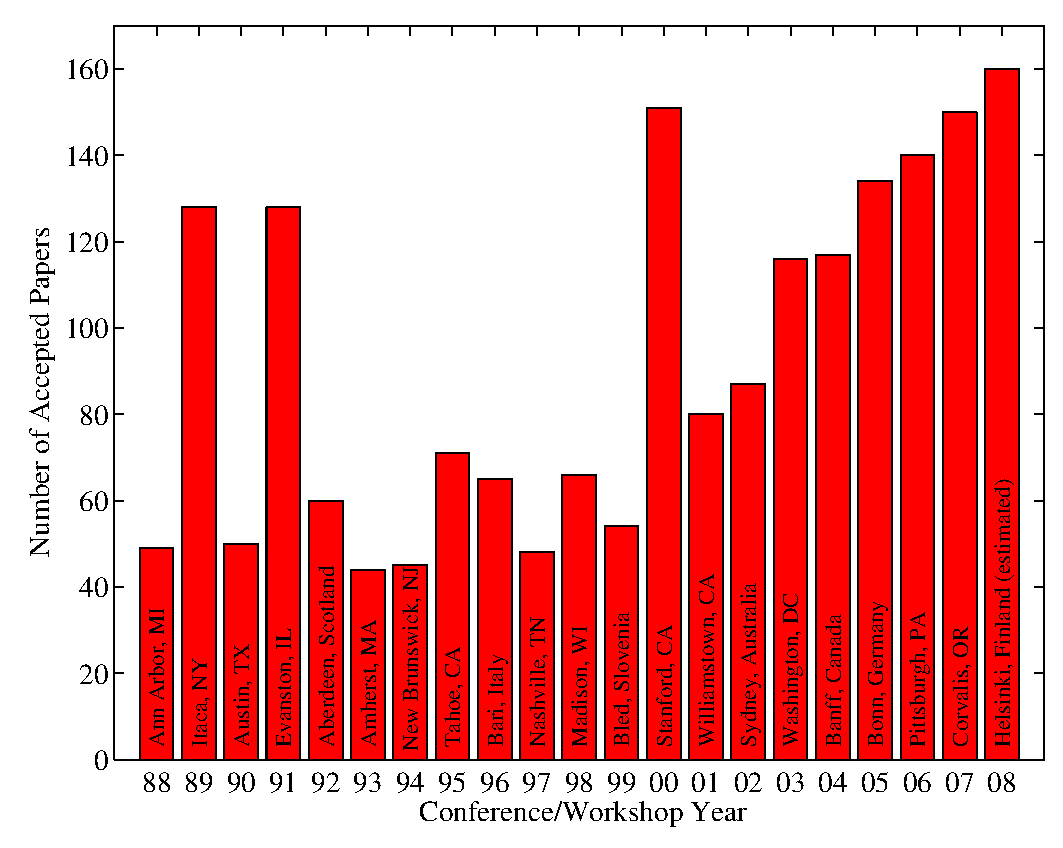
\includegraphics[width=\columnwidth]{figure/icml_numpapers.eps}}
\caption{Historical locations and number of accepted papers for International
Machine Learning Conferences (ICML 1993 -- ICML 2008) and International
Workshops on Machine Learning (ML 1988 -- ML 1992). At the time this figure was
produced, the number of accepted papers for ICML 2008 was unknown and instead
estimated.}
\label{icml-historical}
\end{center}
\vskip -0.2in
\end{figure}

\subsection{Figures}

You may want to include figures in the paper to illustrate
your approach and results. Such artwork should be centered,
legible, and separated from the text. Lines should be dark and at
least 0.5~points thick for purposes of reproduction, and text should
not appear on a gray background.

Label all distinct components of each figure. If the figure takes the
form of a graph, then give a name for each axis and include a legend
that briefly describes each curve. Do not include a title inside the
figure; instead, the caption should serve this function.

Number figures sequentially, placing the figure number and caption
\emph{after} the graphics, with at least 0.1~inches of space before
the caption and 0.1~inches after it, as in
\cref{icml-historical}. The figure caption should be set in
9~point type and centered unless it runs two or more lines, in which
case it should be flush left. You may float figures to the top or
bottom of a column, and you may set wide figures across both columns
(use the environment \texttt{figure*} in \LaTeX). Always place
two-column figures at the top or bottom of the page.

\subsection{Algorithms}

If you are using \LaTeX, please use the ``algorithm'' and ``algorithmic''
environments to format pseudocode. These require
the corresponding stylefiles, algorithm.sty and
algorithmic.sty, which are supplied with this package.
\cref{alg:example} shows an example.

\begin{algorithm}[tb]
   \caption{Bubble Sort}
   \label{alg:example}
\begin{algorithmic}
   \STATE {\bfseries Input:} data $x_i$, size $m$
   \REPEAT
   \STATE Initialize $noChange = true$.
   \FOR{$i=1$ {\bfseries to} $m-1$}
   \IF{$x_i > x_{i+1}$}
   \STATE Swap $x_i$ and $x_{i+1}$
   \STATE $noChange = false$
   \ENDIF
   \ENDFOR
   \UNTIL{$noChange$ is $true$}
\end{algorithmic}
\end{algorithm}

\subsection{Tables}

You may also want to include tables that summarize material. Like
figures, these should be centered, legible, and numbered consecutively.
However, place the title \emph{above} the table with at least
0.1~inches of space before the title and the same after it, as in
\cref{sample-table}. The table title should be set in 9~point
type and centered unless it runs two or more lines, in which case it
should be flush left.

% Note use of \abovespace and \belowspace to get reasonable spacing
% above and below tabular lines.

\begin{table}[t]
\caption{Classification accuracies for naive Bayes and flexible
Bayes on various data sets.}
\label{sample-table}
\vskip 0.15in
\begin{center}
\begin{small}
\begin{sc}
\begin{tabular}{lcccr}
\toprule
Data set & Naive & Flexible & Better? \\
\midrule
Breast    & 95.9$\pm$ 0.2& 96.7$\pm$ 0.2& $\surd$ \\
Cleveland & 83.3$\pm$ 0.6& 80.0$\pm$ 0.6& $\times$\\
Glass2    & 61.9$\pm$ 1.4& 83.8$\pm$ 0.7& $\surd$ \\
Credit    & 74.8$\pm$ 0.5& 78.3$\pm$ 0.6&         \\
Horse     & 73.3$\pm$ 0.9& 69.7$\pm$ 1.0& $\times$\\
Meta      & 67.1$\pm$ 0.6& 76.5$\pm$ 0.5& $\surd$ \\
Pima      & 75.1$\pm$ 0.6& 73.9$\pm$ 0.5&         \\
Vehicle   & 44.9$\pm$ 0.6& 61.5$\pm$ 0.4& $\surd$ \\
\bottomrule
\end{tabular}
\end{sc}
\end{small}
\end{center}
\vskip -0.1in
\end{table}

Tables contain textual material, whereas figures contain graphical material.
Specify the contents of each row and column in the table's topmost
row. Again, you may float tables to a column's top or bottom, and set
wide tables across both columns. Place two-column tables at the
top or bottom of the page.

\subsection{Theorems and such}
The preferred way is to number definitions, propositions, lemmas, etc. consecutively, within sections, as shown below.
\begin{definition}
\label{def:inj}
A function $f:X \to Y$ is injective if for any $x,y\in X$ different, $f(x)\ne f(y)$.
\end{definition}
Using \cref{def:inj} we immediate get the following result:
\begin{proposition}
If $f$ is injective mapping a set $X$ to another set $Y$, 
the cardinality of $Y$ is at least as large as that of $X$
\end{proposition}
\begin{proof} 
Left as an exercise to the reader. 
\end{proof}
\cref{lem:usefullemma} stated next will prove to be useful.
\begin{lemma}
\label{lem:usefullemma}
For any $f:X \to Y$ and $g:Y\to Z$ injective functions, $f \circ g$ is injective.
\end{lemma}
\begin{theorem}
\label{thm:bigtheorem}
If $f:X\to Y$ is bijective, the cardinality of $X$ and $Y$ are the same.
\end{theorem}
An easy corollary of \cref{thm:bigtheorem} is the following:
\begin{corollary}
If $f:X\to Y$ is bijective, 
the cardinality of $X$ is at least as large as that of $Y$.
\end{corollary}
\begin{assumption}
The set $X$ is finite.
\label{ass:xfinite}
\end{assumption}
\begin{remark}
According to some, it is only the finite case (cf. \cref{ass:xfinite}) that is interesting.
\end{remark}
%restatable

\subsection{Citations and References}

If you rely on the \LaTeX{} bibliographic
facility, use \texttt{natbib.sty}
included in the style-file package to obtain reference.

Citations within the text should include the authors' last names and
year. If the authors' names are included in the sentence, place only
the year in parentheses, for example when referencing Arthur Samuel's
pioneering work \yrcite{Samuel59}. Otherwise place the entire
reference in parentheses with the authors and year separated by a
comma \cite{Samuel59}. List multiple references separated by
semicolons \cite{kearns89,Samuel59,mitchell80}. Use the `et~al.'
construct only for citations with three or more authors or after
listing all authors to a publication in an earlier reference \cite{MachineLearningI}.

Use an unnumbered first-level section heading for the references, and use a
hanging indent style, with the first line of the reference flush against the
left margin and subsequent lines indented by 10 points. The references at the
end of this document give examples for journal articles \cite{Samuel59},
conference publications \cite{langley00}, book chapters \cite{Newell81}, books
\cite{DudaHart2nd}, edited volumes \cite{MachineLearningI}, technical reports
\cite{mitchell80}, and dissertations \cite{kearns89}.

Alphabetize references by the surnames of the first authors, with
single author entries preceding multiple author entries. Order
references for the same authors by year of publication, with the
earliest first. Make sure that each reference includes all relevant
information (e.g., page numbers).

Please put some effort into making references complete, presentable, and
consistent, e.g. use the actual current name of authors.
If using bibtex, please protect capital letters of names and
abbreviations in titles, for example, use \{B\}ayesian or \{L\}ipschitz
in your .bib file.
\section*{主旨.}
臺北市立萬芳醫院牙科部設置特殊需求者牙科門診(以下稱特需中心),每週門診2診次,專門服務身心障礙者,牙科櫃台附有身心障礙服務窗口,設置志工,與負責身心障礙門診之牙科輔助人員共同幫忙引導、溝通、協助患者就醫。候診區及初診區均有輪椅無障礙空間。
%先申請特需中心,然後牙科部專任醫師才具有到宅牙醫服務的資格,當然也需要身障照護的學分。到宅小組需要一名醫師、一名護理師,攜帶必要設備,每一名案主收案都事先申請核可
特殊需求者的口腔照護,因日常生活打理由照顧者代勞,往往無法顧及基本的口腔衛生照護,在宅臥床患者更面臨齲齒、牙周病細菌感染的重大危機,因其就醫之阻礙甚多,四、五層樓之公寓往往沒有電梯。
特需中心配合長照2.0政策,規畫居家牙醫醫療服務。

\section*{依據.}
%「全民健康保險會」協定年度醫療給付費用總額事項」辦理
% https://www.nhi.gov.tw/BBS_Detail.aspx?n=73CEDFC921268679&sms=D6D5367550F18590&s=DC5108C6E3DD21D0
「111年全民健康保險牙醫門診總額特殊醫療服務計畫」辦理「特殊需求者口腔醫療與保健推廣計畫」(以下稱本計畫)。

\section*{目的.} 旨在提升特定身心障礙者牙醫醫療服務品質,並加強口腔保健。

\section*{方法.}
%\section{計畫種類}
\section{特殊需求者牙科醫療服務計畫}

\subsection{醫院牙醫醫療服務(以下稱到院牙醫服務)}
\label{dent}

\subsubsection{特需中心}

\begin{outline}

%\1 衛生福利部「特殊需求者牙科醫療服務示範中心獎勵計畫」之醫院 
%or 「特殊需求者牙科醫療服務示範中心獎助計畫」及「特殊需求者牙科醫療服務獎助計畫」申請補助作業
\1 初級照護院所:
台北市立萬芳醫院-委託
財團法人私立台北醫學大
學辦理(醫事機構代號1301200010),審核已通過1110101至1111231。
% https://cda.org.tw/cda/public_medical_institution_type_b_search_result.jsp
%(1)申請書格式如【附件3】。 %(2)身心障礙教育訓練之學分證明影本。
%(3)牙醫師證書正反面影本一份。
\2 醫院資格
%    \3 可施行鎮靜麻醉之醫療院所及提供完備醫療之醫護人員。
    \3 設備需求:牙科門診應有急救設備、氧氣設備。
    %、麻醉機、心電 圖裝置(Monitor,包括血壓、脈搏、呼吸數之監測、血氧濃度pulse oximeter)、無障礙空間及設施(詳【附表】)。
%    \3 需1位以上具有從事相關工作經驗之醫師。
\2 醫師資格
    \3 %2位以上具有從事相關工作經驗之醫師,負責醫師自執業執照取得後滿5年以上之臨床經驗,其他醫師
    自執業執照取得後滿1年以上之臨床經驗之醫師。
    \3 經身心障礙口腔醫療教育課程(詳\ref{certificate})訓練合格。

\1 進階照護院所 %進階照護院所:口腔醫療與保健推廣計畫書
\2 醫院資格
    \3 可施行鎮靜麻醉之醫療院所及提供完備醫療之醫護人員。
    \3 設備需求:牙科門診應有急救設備、氧氣設備、麻醉機、心電 圖裝置(Monitor,包括血壓、脈搏、呼吸數之監測、血氧濃度pulse oximeter)、無障礙空間及設施(詳【附表】)。
%    \3 需2 位以上具有從事相關工作經驗之醫師。
\2 醫師資格
    \3 2位以上具有從事相關工作經驗之醫師,負責醫師自執業執照取得後滿5年以上之臨床經驗,其他醫師自執業執照取得後滿1年以上之臨床經驗。
    \3 經身心障礙口腔醫療教育課程(詳\ref{certificate})訓 練合格。
\end{outline}

\subsubsection{申請方式}
\begin{outline}

\1 全民健康保險牙醫門診總額特殊醫療服務計畫牙醫醫療服務加入申請書(院所內服務/到院牙醫服務)【附件3】
\1 全民健康保險牙醫門診總額特殊醫療服務計畫院所申請流程圖【附件7】
\1 牙科進階照護院所友善醫療環境評量(詳【附表】)

\end{outline}

%\subsection{醫療團牙醫醫療服務}
%x (七)(到身心障礙福利機構)
%因本計畫醫療團成立的規定,護理之家僅限定照護司擇定之2家,目前無法新增。另醫療團主要服務機構內符合本計畫特定障別之患者,因其困難外出就醫,故組成醫療團至機構內服務。而貴院所屬護理之家已在萬芳醫院內,就醫方便,建議循一般就診方式處理。

%以醫療團為單位,申請時應檢附下列資料:(含特定需求者牙醫醫療服務){申請書格式【附件5】、牙醫師公會評估表【附件6】、護理之家(由衛生福利部護理及健康照護司擇定)之立案證明、同意函、簡介、收容對象名冊、口腔狀況、牙科設備、 醫師服務排班表、牙科治療計畫、維護計畫、口腔衛生計畫、經費評估、牙醫師證書正反面影本乙份等}

\subsection{居家牙醫醫療服務(以下稱到宅牙醫服務)}
% (八)居家牙醫醫療服務 (p15-18)

\subsubsection{服務對象:}
\begin{outline}
\0 限居住於住家(不含照護機構)的牙醫特殊需求病人,需符合下列條件之一:
    \1 全民健康保險居家醫療照護整合計畫之居家醫療、重度居家醫療及安寧療護階段之病人,且有明確之牙醫醫療需求。
    \1 出院準備及追蹤管理費(02025B)申報病人,且有明確之牙醫醫療需求。
    \1 特定身心障礙者,清醒時百分之五十以上活動限制在床上或椅子上,且有明確之牙醫醫療需求。前述特定身心障礙者之障礙類別(詳【附件2】)包含:
        \2 肢體障礙(限腦性麻痺、腦傷及脊髓損傷之中度肢體障礙、及重度以上肢體障礙)
        \2 重度以上視覺障礙、重度以上重要器官失去功能
        \2 中度以上之植物人、智能障礙、自閉症、精神障礙、失智症、頑固性(難治型)癲癇
        \2 因罕見疾病而致身心功能障礙、染色體異常、發展遲緩兒童
        \2 其他經主管機關認定之障礙(須為新制評鑑為第1、4、5、6、7類者)
        \2 多重障礙(或同時具備二種及二種以上障礙類別)

    \1 「失能老人接受長期照顧服務補助辦法」之補助對象(以下稱失能老人),並為各縣市長期照顧管理中心之個案,且因疾病、傷病長期臥床的狀態,清醒時百分之五十以上活動限制在床上或椅子上,行動困難無法自行至醫療院所就醫之病人。

\end{outline}

\subsubsection{服務流程(詳【附件18】)}
\label{certificate}


% Set spacing between columns
\setlength{\tabcolsep}{8pt}

% Set the width of each column
\begin{longtable}{p{1.3in}p{4.8in}}

%\color{OliveGreen}{收案條件}
% & 限居住於住家(不含照護機構)且符合下列條件之一者:全民健康保險居家醫療照護整合計畫之居家醫療病人(重度或極重度特定身心障礙者)、安寧療護階段之病人、出院準備及追蹤管理費(02025B)申報病人、失能老人(為各縣市長期照顧管理中心之個案)。 \\
\color{OliveGreen}{事前申請}
 & 首次訪視申請表【附件15】、後續追蹤治療計畫【附件16】均須註明後送轉診醫院。經牙醫全聯會核可後,始得至案家提供牙醫醫療服務。 \\
 
\color{OliveGreen}{醫師資格}
& 已參加本計畫照護院所(詳\ref{dent})之專任醫師。
自執業執照取得後滿1年以上臨床經驗之醫師。每位醫師首次加入本計畫,須接受6學分以上身心障礙口腔醫療業務等相關之基礎教育訓練(\underline{須包含居家牙醫醫療之相關學分})。加入計畫後,每年須再接受4學分以上之身心障礙口腔醫療業務相關之再進修教育課(每年再進修課程不得重複);本計畫之醫師須累積七年以上且超過30(含)學分後,得繼續執行計畫,惟課程皆須由中華牙醫學會或牙醫全聯會認證通過。 \\

\color{OliveGreen}{到宅小組}
 & 一名醫師搭配一名護士出診; 須有熟悉該患者狀況的人員(家屬)陪同就診。護理人員至病人住家提供醫療服務,須依法令規定事前報經當地衛生主管機關核准。符合醫師法所稱應邀出診,醫師不需經事先報准。\\
 
\color{OliveGreen}{就診文書}
& 醫師應於院所製作電子病歷留存,且須將病人身分影印本及計畫所須之證明文件,黏貼於病歷首頁後掃瞄為電子檔 留存,以備查驗。就診紀錄【附件12】應詳實紀錄。侵入性治療應取得病人家屬或監護人之書面同意書。\\
 
\color{OliveGreen}{攜帶設備}
& 生理監測器(血壓、血氧)、攜帶式洗牙機、攜帶式強力抽吸設備與抽痰管、牙科治療器械、有效的急救設備(人工氣道 laryngeal mask airway, LMA)、氧氣設備(含氧氣幫浦、氧氣筒須有節流裝置、氧氣面罩等)、急救藥品、開口器及健保卡讀寫卡設備等相關物品。\\

\color{OliveGreen}{照護內容}
& 基於安全考量,居家牙醫醫療服務時,以提供牙周病緊急處理、牙周敷料、牙結石清除、牙周暨齲齒控制基本處置、塗氟、(非)特定局部治療、簡單性拔牙及單面蛀牙填補等服務為限。居家牙醫醫療服務給付項目及支付標準詳【附件17】。醫護人員宜針對案主的情況,善盡指導案家清潔口腔的責任。\\

\color{OliveGreen}{病人安全}
& 診療期間隨時注意病人之生理及心理狀況。若遇臨時緊急狀況或危急情形,應初步保護呼吸道,並立刻和計畫中最近的後送醫院聯絡,進行緊急醫療及後送程序。\\


\color{OliveGreen}{感染管制}
& 牙醫醫療服務應符合「牙醫巡迴醫療、特殊醫療、矯正機關之牙醫服務感染管制 SOP 作業細則」【附件14】。設備之維護、清潔保養及醫療廢棄物由醫療院所依相關法規妥善處理。\\

\color{OliveGreen}{部分負擔}
& 依牙醫門診基本部分負擔向案家計收。\\

\color{OliveGreen}{醫療費用}
& 特約醫事服務機構執行本計畫之醫療費用應按月申報給付項目【附件17】,並於門診醫療服務點數清單依下列規定填報「案件分類」及「特定治療項 目代號」欄位,案件分類 16,特定治療項目代號(一)請依病人類 別填報【極重度FS、重度FY、中度 L4、發展遲緩兒童LE、失能老人L2、居整病人LC、出院準備LD、腦傷及脊髓損傷之中度肢體障礙:LJ】。醫令類別為
「4 不得另計價之藥品、檢驗(查)、診療項目或材料」。\\



\color{OliveGreen}{相關規範}
%\begin{outline}
& 個案首次接受居家牙醫醫療服務(含訪視)前,牙醫師須檢送申請
表【附件15】至牙醫全聯會,由牙醫全聯會於每月 20 日前將核可 名單函送保險人分區業務組備查。個案於首次接受居家牙醫醫療服 務(含訪視)後,須於次月 20 日前檢送病人之「口腔醫療需求評 估及治療計畫」【附件16】,正本送所屬保險人分區業務組、副本送 牙醫全聯會備查。經催繳三個月內仍未改善者,經保險人分區業務 組及牙醫全聯會確認,得暫停執行居家牙醫醫療服務。


%\end{outline}

\end{longtable}


%%%%
%到院牙醫服務
%到宅牙醫服務
\subsection{到宅牙醫服務}
%\label{certificate}


% Set spacing between columns
\setlength{\tabcolsep}{8pt}

% Set the width of each column
\begin{longtable}{p{1.3in}p{4.8in}}

%\color{OliveGreen}{收案條件}
% & 限居住於住家(不含照護機構)且符合下列條件之一者:全民健康保險居家醫療照護整合計畫之居家醫療病人(重度或極重度特定身心障礙者)、安寧療護階段之病人、出院準備及追蹤管理費(02025B)申報病人、失能老人(為各縣市長期照顧管理中心之個案)。 \\
\color{OliveGreen}{人力須求}
 & 限執照登記於院所,且合乎本計畫之醫師(詳\ref{certificate}),及特殊需求牙科負責護士一名(以下簡稱專責護士)組成到宅小組。並可以帶領PGY醫師出診,為社區牙醫服務及教學。\\
 %; 須有熟悉該患者狀況的人員(家屬)陪同就診。護理師至病人住家提供醫療服務,則須依法令規定事前報經當地衛生主管機關核准。因符合醫師法所稱應邀出診,不需經事先報准。\\
%& 已參加本計畫照護院所(詳\ref{dent})之專任醫師。
%自執業執照取得後滿1年以上臨床經驗之醫師。每位醫師首次加入本計畫,須接受6學分以上身心障礙口腔醫療業務等相關之基礎教育訓練。加入計畫後,每年須再接受4學分以上之身心障礙口腔醫療業務相關之再進修教育課(每年再進修課程不得重複);本計畫之醫師須累積七年以上且超過 30(含)學分後,得繼續執行計畫,惟課程皆須由中華牙醫學會或牙醫全聯會認證通過。 \\
 
\color{OliveGreen}{服務內容}
 & 專責護士準備事前審查文件,首次訪視(表【附件15】),經牙醫全聯會核可後,安排家訪。家訪時經醫師與案家同意後收案,方可安排一次治療或定期追蹤治療(計畫詳【附件16】)。醫師於治療(項目詳【附件17】)後須製作電子病歷及就診紀錄(【附件12】)。侵入性治療應取得病人家屬或監護人之書面同意書(依院所格式)。每次到訪均須指導案家清潔口腔的技巧。\\

\color{OliveGreen}{計畫期程}
& 自每年核可後,至當年12月31日。\\
 
\color{OliveGreen}{服務場所}
%到院牙醫服務
& 專責護士與案家排定日期時段(宜在案主進食前),到宅小組到宅服務時,可按車程距離收取車馬費。一診次可安排一至三家,每名醫師一週出診以二次為限。\\

\color{OliveGreen}{設備須求(詳【附件19】)} % Tex's 設備表 ABC
& 專責護士打包整理設備,包括個人防護、生理監測器(血壓、血氧)、攜帶式洗牙機、攜帶式強力抽吸設備與抽痰管、牙科治療器械、有效的急救設備(人工氣道 laryngeal mask airway, LMA)、氧氣設備(含氧氣幫浦、氧氣筒須有節流裝置、氧氣面罩等)、急救藥品、開口器及健保卡讀寫卡設備等相關物品。宜考量行李總重量,許多四、五樓層住宅並沒有電梯。\\


% DOH_equip.tex

%\color{OliveGreen}{計畫經費} & \\
%「特殊需求者牙科醫療服務示範中心獎助計畫」及「特殊需求者牙科醫療服務獎助計畫」申請補助作業,申請期限為自公告日起20天(即至110年2月17日止)。
%\url{https://www.mohw.gov.tw/cp-18-57852-1.html}
%\url{https://www.cda.org.tw/cda/news_detail.jsp?nid=2255}\\
% 申請機構資格:經衛生局指定開設身心障礙者特別門診之醫院(該院應設有牙科及發展遲緩療育特別門診)
% 補助醫院:計畫期間達成應辦理事項者,得請領補助費用計新臺幣(以下同)40萬元整;如每周開設特別門診達3診(含)以上,與至少8家醫療機構(其中3家需為未合作過之新增名單)建置轉診機制,並訪視機構達12場以上(離(外)島及台東縣之承作醫院如每週開設特別門診達2診(含)以上,與至少4家醫療機構(其中1家需為未合作過之新增名單)建置轉診機制,並訪視機構機構達1場以上),額外給予補助費用計10萬元整,每家醫院以50萬元為補助上限。
% 第(二)項:補助醫師提供特殊需求者牙科照護服務
%每一特定障礙類別之服務人次給予補助費用計1,000點,惟病人當次僅單純接受牙結石清除(洗牙)處置者,該人次僅給予補助費用計500點,單次最多1,000點。
%各醫院於計畫申請書載明,年度預估申請補助金額,由本部年度結案時,依各院實際服務人次,採總額搭配點值(每點至多1元)方式,核實撥付。
% 108年辦理「特殊需求者牙科醫療服務獎勵計畫」補助全國共22家一般醫院,每週開設特殊需求門診計143診以上,累計服務人次至11,765人次。

%& 基於安全考量,居家牙醫醫療服務時,以提供牙周病緊急處理、牙周敷料、牙結石清除、牙周暨齲齒控制基本處置、塗氟、(非)特定局部治療、簡單性拔牙及單面蛀牙填補等服務為限。居家牙醫醫療服務給付項目及支付標準\\
\end{longtable}


%
\section{牙醫特殊計畫承辦窗口}
\noindent 社團法人中華民國牙醫師公會全國聯合會\\
牙醫特殊計畫承辦人朱智華\\
104台北市中山區復興北路420號10樓\\
電話:02-25000133 ext. 262\\
傳真:02-25000126\\
uase@cda.org.tw\\
% my project main text
%
\section*{Acknowledgements}

Acknowledgements is an unnumbered section at the end of the paper. Typically, this will include thanks to colleagues who contributed to the ideas, and to funding agencies and corporate sponsors that provided financial support.


%\bibliographystyle{plainnat}
%\bibliography{ref}

\newpage
\appendix
%
\section{You \emph{can} have an appendix here.}

You can have as much text here as you want.


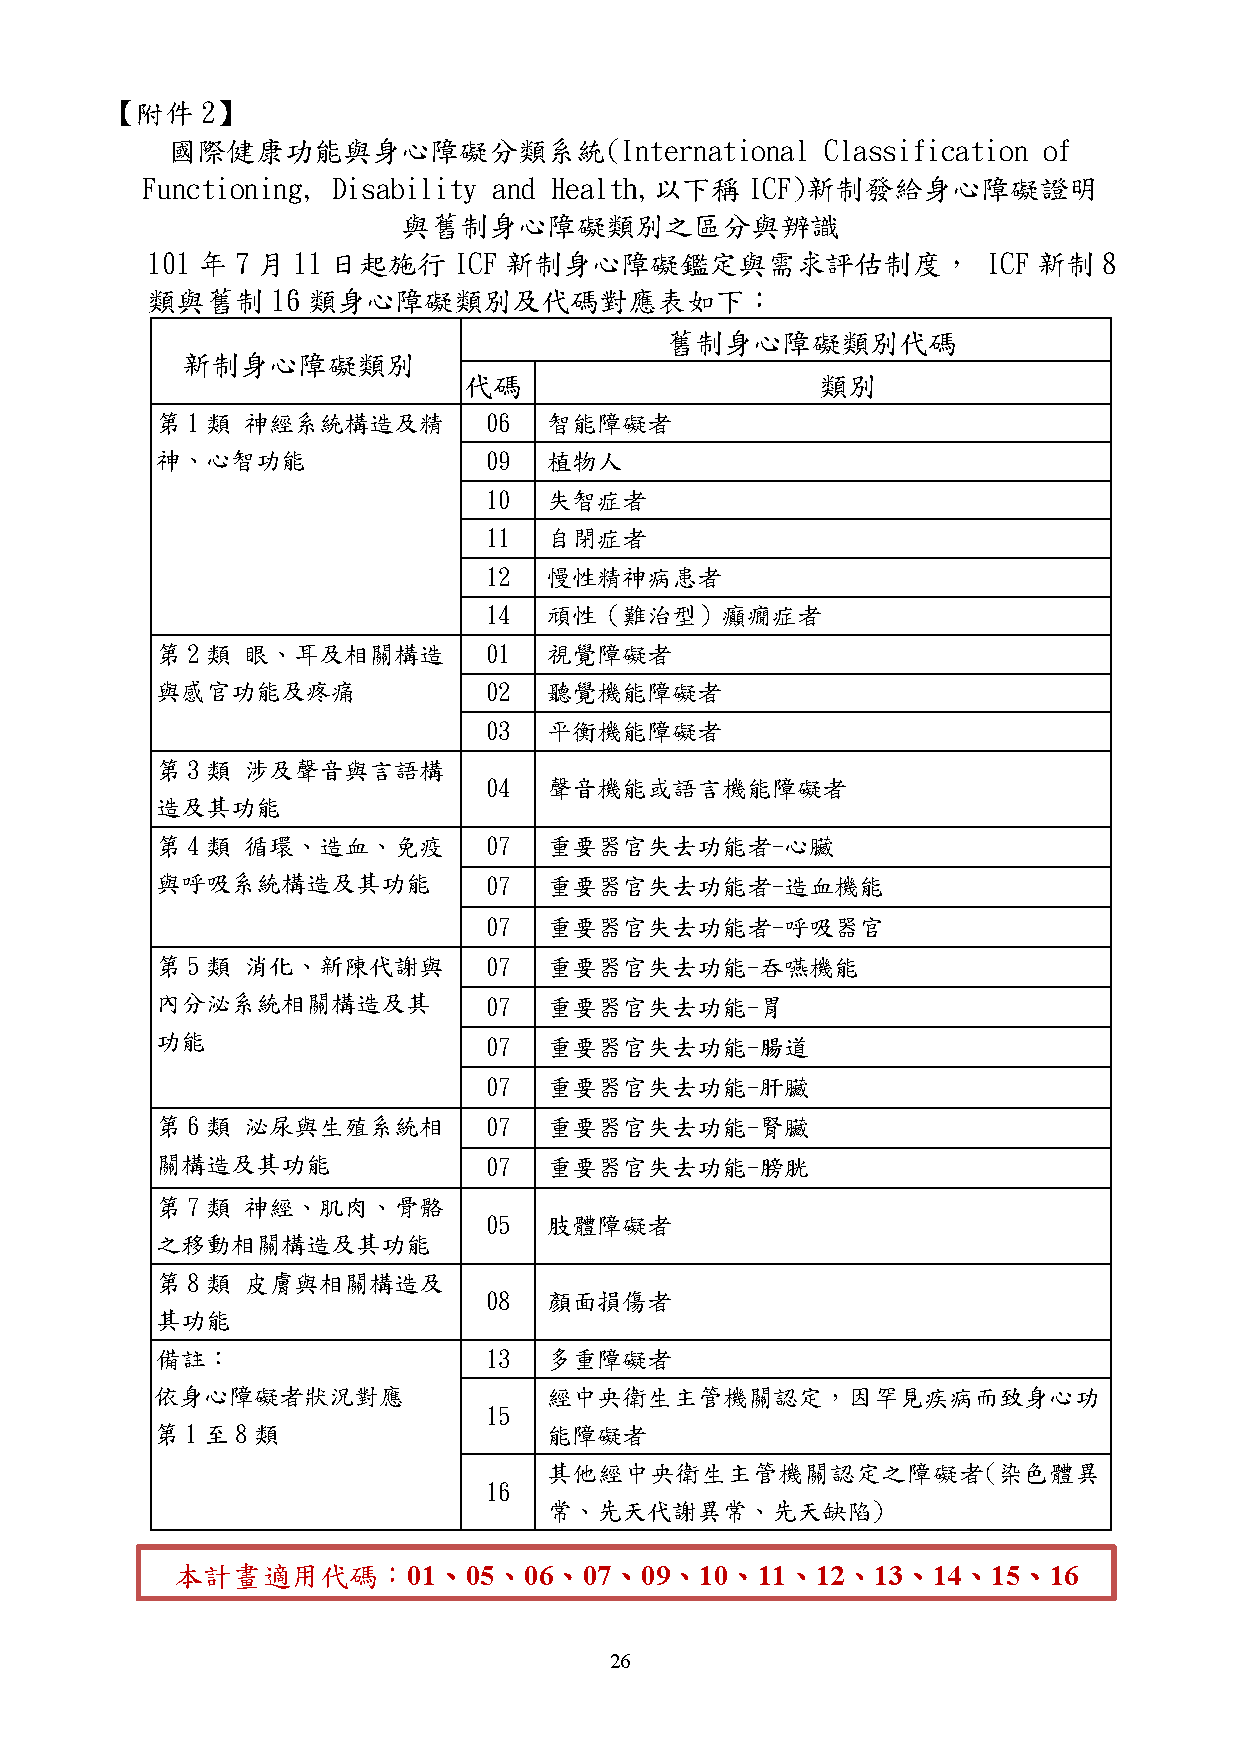
\includepdf[pages=-]{111年牙醫特殊醫療服務計畫 (ICF).pdf}
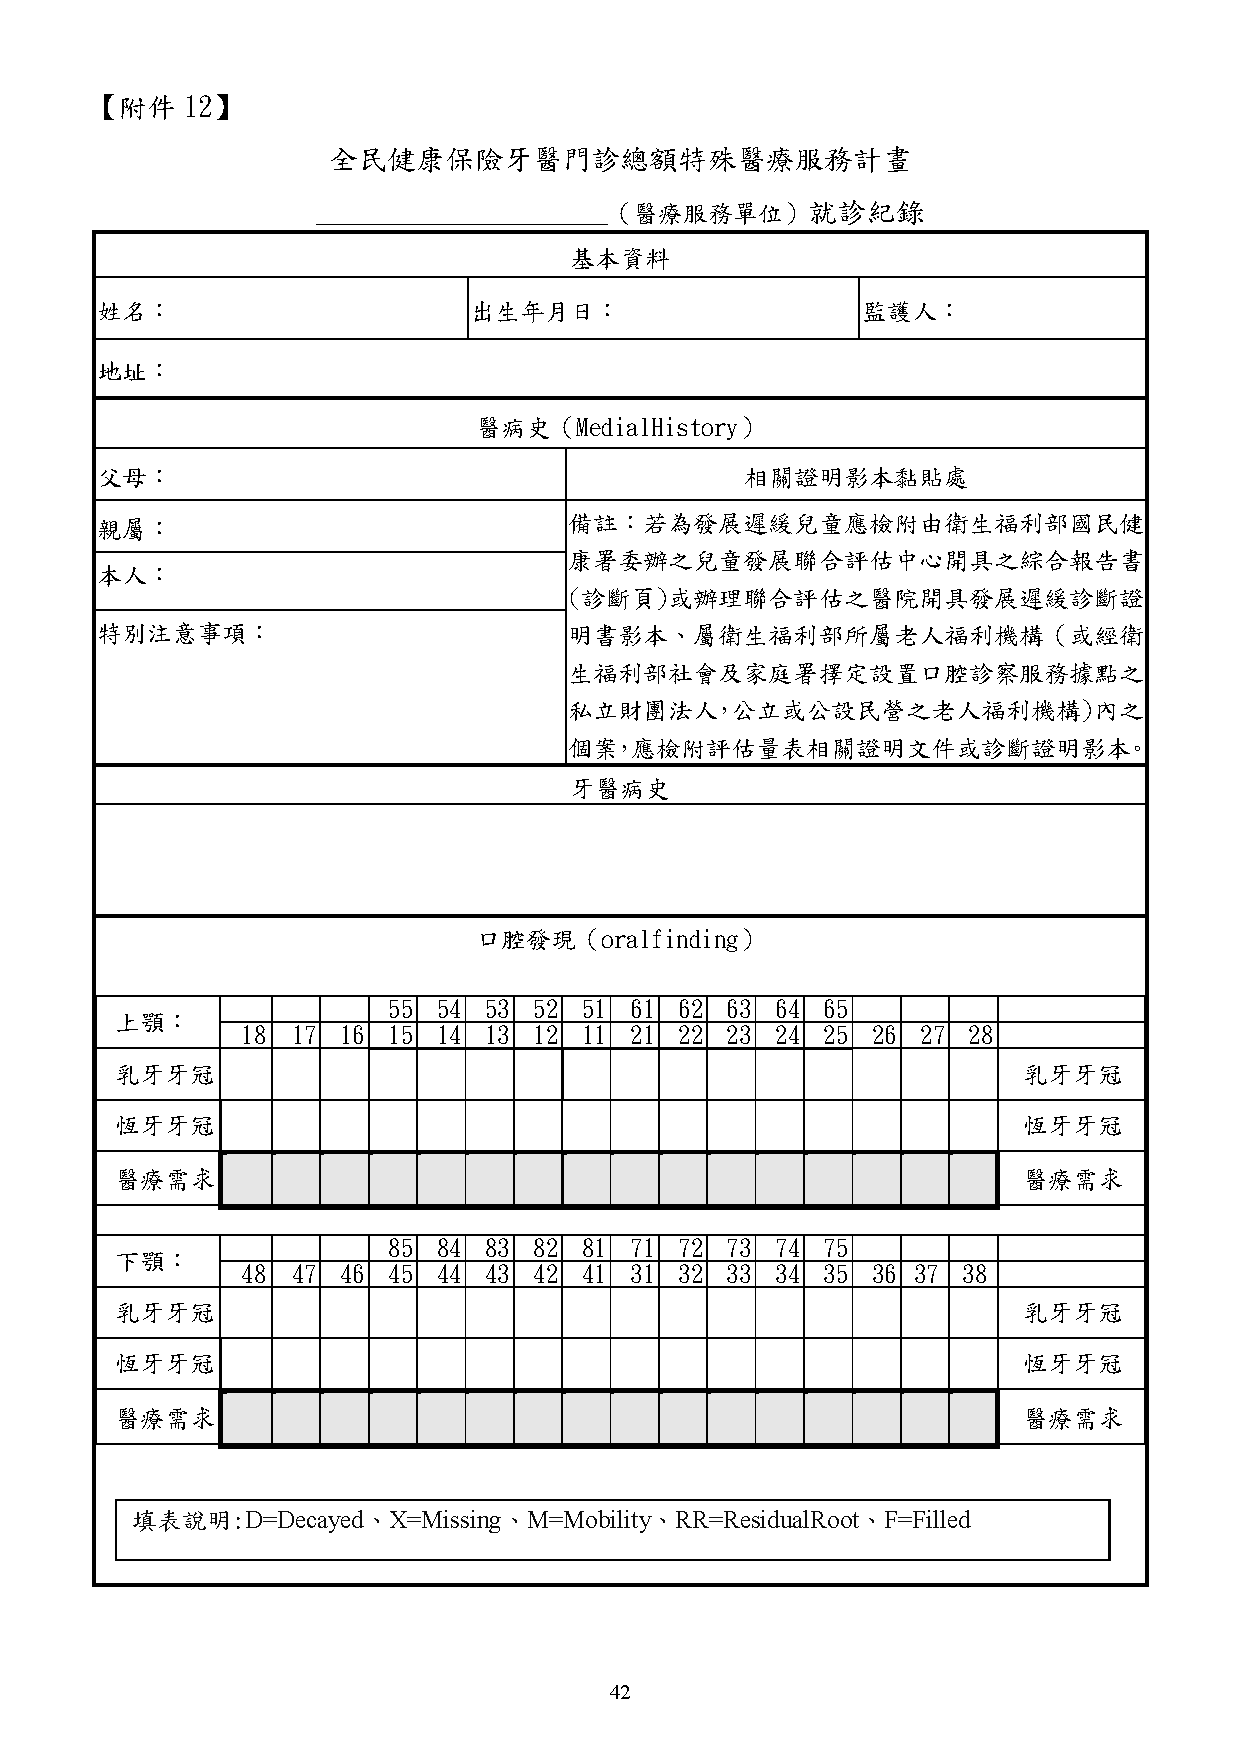
\includepdf[pages=-]{111年牙醫特殊醫療服務計畫 (附件12).pdf} % 附件12 診紀錄
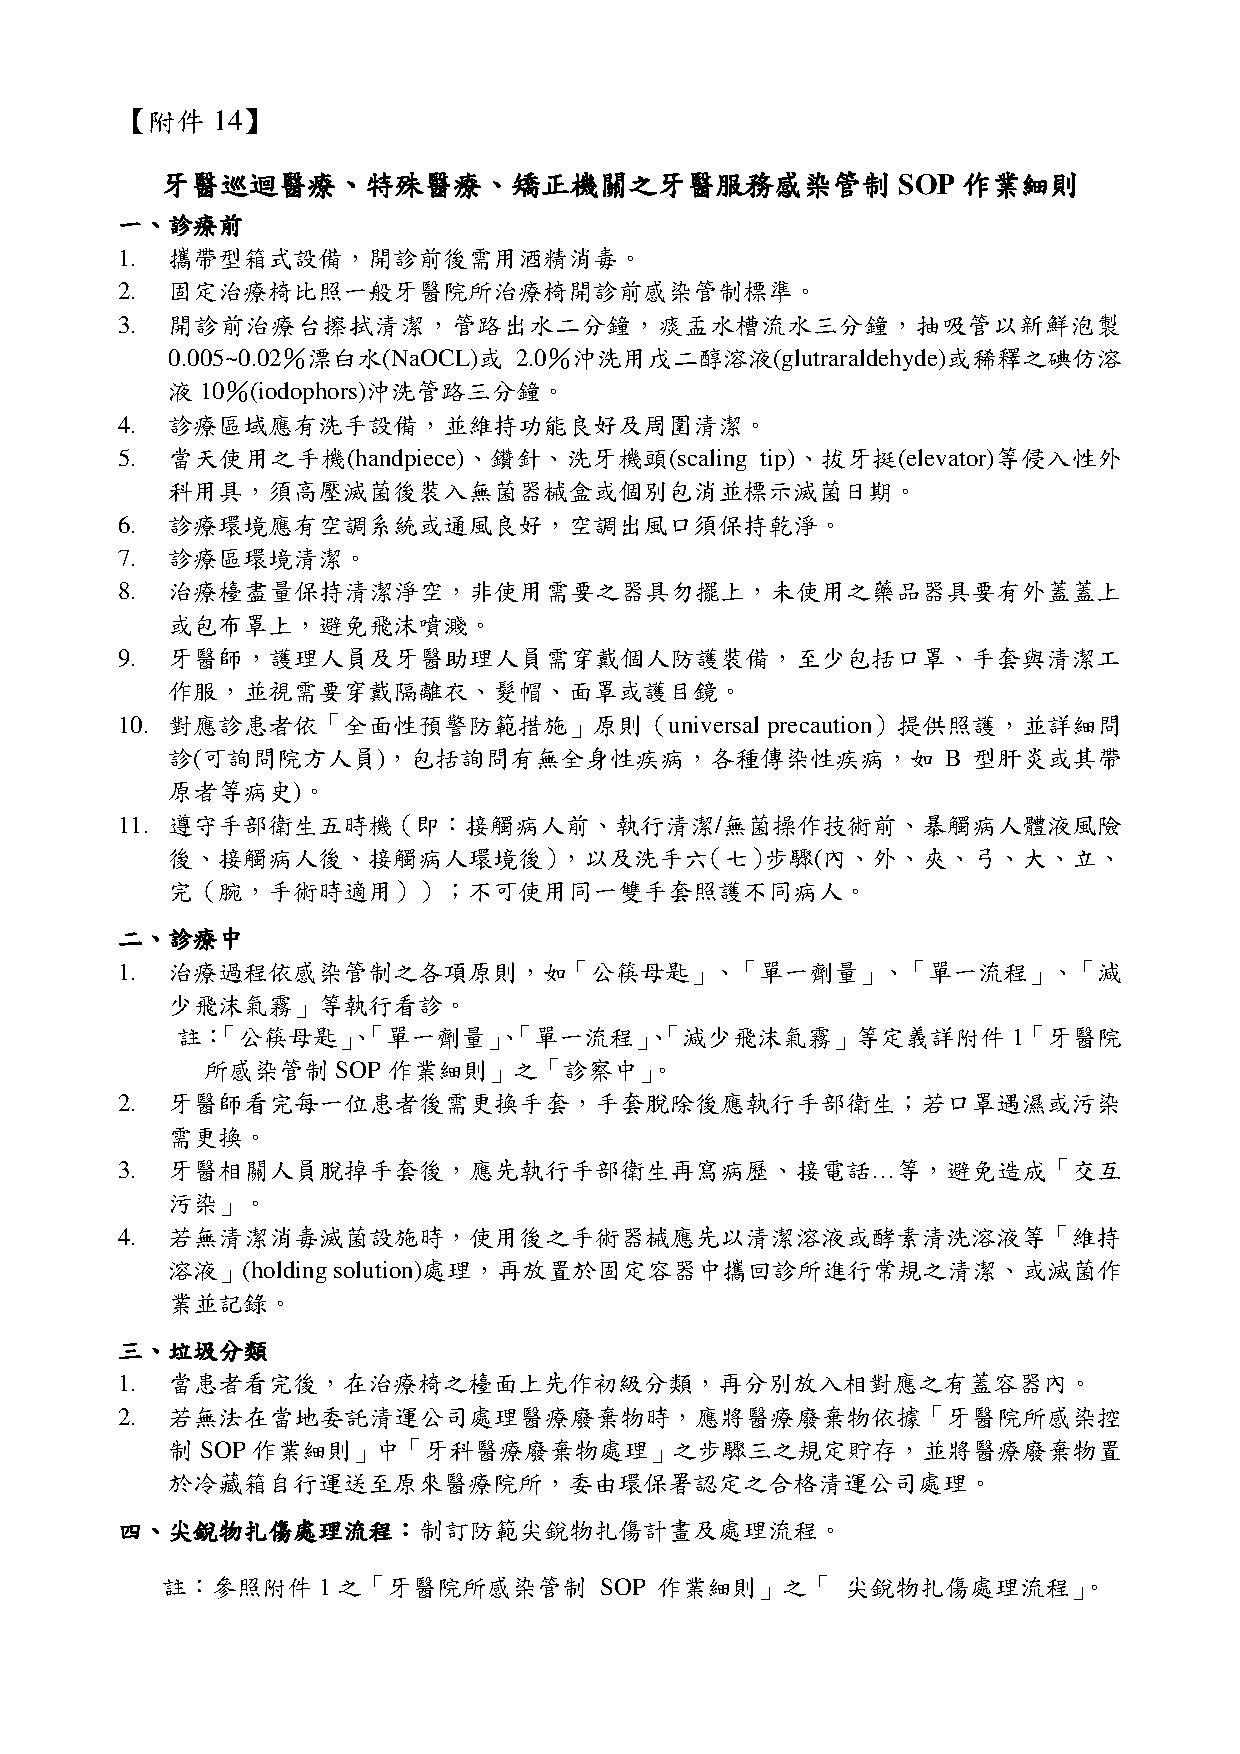
\includepdf[pages=-]{A040170081040500-1090331-7000-014.pdf} % 附件14
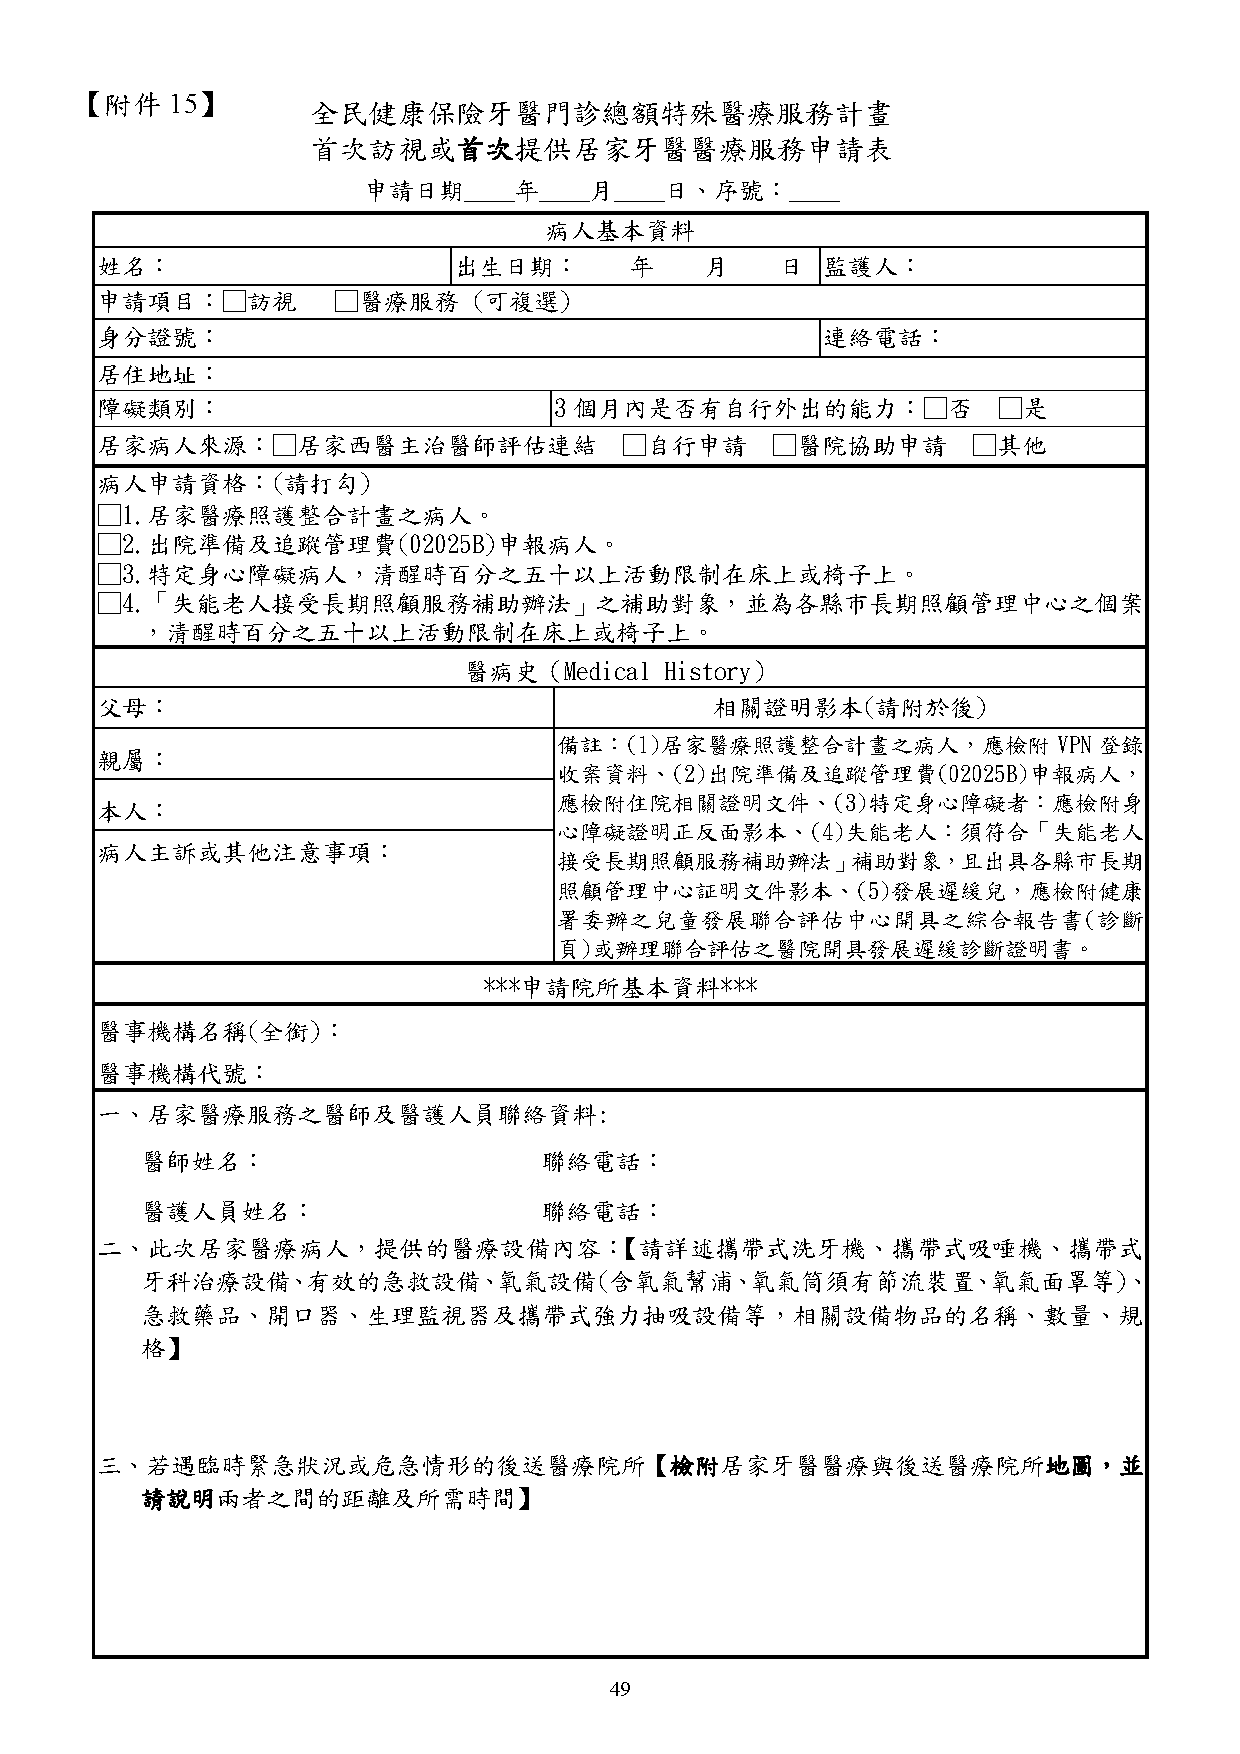
\includepdf[pages=-]{111年牙醫特殊醫療服務計畫 (DOH_附件).pdf}

\end{document}



%%% a list in TMWH
到宅牙醫醫療服務已納入「全民健康保險居家醫療照護整合計畫」中
%https://cda.org.tw/cda/public_medical_institution_type_b_search_result.jsp

02-29307930*7088王秘書 116 台北市文山區興隆路3段111號2樓轉牙科
台北市立萬芳醫院-委託財團法人私立台北醫學大學辦理

王柏翔
卓郁純
林光勳
翁瑛祺
許晶晶
陳育德
陳俊銘
陳培惠
黃培琪
黃曉楓
蔡昀潔
謝承祐 